\section{Software Process Notation --- TODO by 0000 13th August 2013} \label{notation}

In Section \ref{introduction}, we briefly discussed the idea of classifying and comparing models.
As we further noted, the different process descriptions make classification and comparison of
development processes difficult.
Thus, we introduce a standardised notation that will allow us to describe and discuss software
processes in an unambiguous manner.\\
\\
To a reader interested in the notation used throughout the paper, we direct them
to \FIXME which summarises the graphical notations we have
designed.
It gives the natural language meaning and semantics of each of the symbols we employ.\\
\\
Otherwise, this chapter introduces our graphical notation by justifying each symbol we
use.
We draw inspiration from UML Activity Diagrams \cite{Dumas01umlactivity,BellUMLBasics}, as well as
the notation Woodings describes in \ref{Woodings2013Tut1}.
We discuss the design and ideas behind our notation, and why we believe it is a
good notation system.
\subsection{Notation}

In \cite{fuggetta2000software} we define a process as
\begin{quote}
A software process can be defined as the coherent set of policies, organizational structures,
	technologies, procedures, and artifacts that are needed to conceive, develop, deploy, and maintain
	a software product.
\end{quote}

From this definition, we can note that we must be able to at least denote four things
\begin{itemize}
	\item a point at which the set of policies and technologies should begin deployment
	\item a point at which the policies and technologies should cease operation on the software
	product development
	\item sub-tasks to arbitrarily divide the component procedures of a process into as fine detail as
	is necessary
	\item inputs and outputs which are the artifacts used within a software development process
\end{itemize}

We first introduce the entry and exit points of a process; these are the points where it starts and
ends.

\begin{figure}[h!]
\centering
\begin{subfigure}[b]{.45\textwidth}
\centering

\includegraphics[scale=0.6]{media/Entry}
\caption{The entry point in the program.}
\label{entryFigure}
\end{subfigure}
~
\begin{subfigure}[b]{.45\textwidth}
\centering

\includegraphics[scale=0.6]{media/Exit}
\caption{The exit point of the program.}
\label{exitFigure}
\end{subfigure}
\caption{Here, we show our notation for the entry and exit points of a process.
Note that it is quite similar to notation in \ref{Dumas01umlactivity} for
  signifying where a process begins and ends.}
\label{entryExitFigure}
\end{figure}

Without knowing where we start and end, our process is a never-ending sequence of tasks, which
either has no recognisable place to start or no point to recognise the software product as
``finished".
This is counter-intuitive to the purpose of a process which is to construct a software product.\\
\\
Next, we define a sub-task.
As we noted in our previous definition, there are sub-procedures which make up our process.

\begin{figure}[h!]
\centering
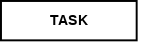
\includegraphics[scale=0.6]{media/Task}
\caption{A single task of a process.}
\label{taskFigure}
\end{figure}

In \cite{Woodings2013Tut1}, Woodings comments on the need to break down a
process into tasks.
A process that consists of a single task is pointless, as it offers no new
insights into the innards and comparability of a process.\\
\\
Thus, a single task must act on {\em something}, and as a result of its actions
it must produce something different.
To denote dependencies upon inputs or other tasks, we use arrows, whilst we denote tangible outputs
from a task with a circle.

\begin{figure}[h!]
\centering
\begin{subfigure}[b]{.45\textwidth}
\centering
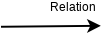
\includegraphics[scale=0.6]{media/Dependency}
\caption{The arrow denotes a dependency of one task on another. As an example, suppose $A \to B$.
	Then $B$ is dependent on $A$.
We can add further detail to this dependency by labelling the relation.}
\label{depFigure}
\end{subfigure}
~
\begin{subfigure}[b]{.45\textwidth}
\centering
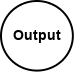
\includegraphics[scale=0.6]{media/Output}
\caption{This circle denotes the output from a task, but also the input to another task. It
is logical that each output is used as the input of {\em some} point in the process (including the
		exit point), otherwise the output itself has no usage.}
\label{outputFigure}
\end{subfigure}
\caption{An arrow will show dependency and a circle shows the output of a task,
which also denotes the input for some point in the process.} \label{depOutFigure}
\end{figure}

Note that we have said that \ref{outputFigure} denotes either an input or an
output.
We note that although an output must implicitly be an output to some other
process point, inputs need not necessarily be generated from a task.
Similarly, we do not make the claim that all tasks require inputs, only that
they must generate some output.\\
\\
Processes may branch at certain points due to needing to make a decision on the conditions of the
process and the appropriate path the process should take to complete development.
We will call these ``decision points".
At other times, tasks can be parallelised between members of the software development team.

\begin{figure}[h!]
\centering
\begin{subfigure}[b]{.45\textwidth}
\centering

\includegraphics[scale=0.6]{media/Parallelised}
\caption{The above notation symbolises that multiple tasks should begin occurring in parallel (that
		is, simultaneously).}
\label{parFigure}
\end{subfigure}
~
\begin{subfigure}[b]{.45\textwidth}
\centering
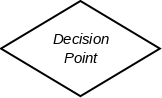
\includegraphics[scale=0.6]{media/Branching}
\caption{The following is a decision point, where multiple paths can emerge from this single point.}
\label{branFigure}
\end{subfigure}
\end{figure}

\pagebreak %TODO: Check if pagebreak is good idea

Finally, we pay a special attention to the verification process.
Verification that a task is correct and its outputs meet the requirements and standards expected by a client
and other software maintainers is, in itself a process.
We separate our notation of verification to thus distinguish it as a ``shadow" or ``reflection"
procedure of a task (or sequence of tasks).

\begin{figure}[h!]
\centering
\begin{subfigure}[b]{.45\textwidth}
\centering

\includegraphics[scale=0.6]{media/BeginVerification}
\end{subfigure}
~
\begin{subfigure}[b]{.45\textwidth}
\centering
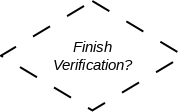
\includegraphics[scale=0.6]{media/EndVerification}
\end{subfigure}
\caption{Here, verification is treated as its own subprocess. The notation has the same meaning as
	\ref{taskFigure} or \ref{branFigure}, except restricted to the verification process.
	However, its dotted-line distinction is
	two-fold; it is the ``shadow" process to ensure that a task has been completed correctly, but is
		also treated in an ad-hoc and almost ``optional" manner by organisations.
		Thus it is not a ``solid" or ``defined" process like \ref{taskFigure} or \ref{branFigure}.}
\label{verification}
\end{figure}

\subsection{Design}

The Object Modelling Group (OMG) specifies in \ref{bpmnfaq} that their Business Process Modelling Notation
specifies ``the sequence of processes and messages" that are passed during a related set of
activities.\\
\\
More importantly, \ref{bpmnfaq} states that a business user or manager ``should be able to easily
understand a BPMN business process diagram."
Conversely, a process implementer or reviewer ``should be able to adorn BPMN with further detail to
represent the process in a physical implementation."\\
\\
We are converging on a set of criteria with which to judge a notation and argue for its usefulness,
but as of yet our quotes have not explicitly stated what we want out of a notation.
Woodings (in \ref{Woodings2013Tut1}) extends the implications stated by the OMG, by listing three criteria for a notation
\begin{enumerate}
	\item simple, or easily understandable by a reader \label{simpleNot}
	\item detailed, and thus conveying enough meaning to a reader to implement and follow
	a process \label{detailedNot}
	\item complete, shows all essential features of a process \label{completeNot}
\end{enumerate}

We will address our notation with respect to each of the three criteria separately.
Firstly, we note that our notation is limited, with only nine different symbols.
Each symbol within our notation has a well-defined semantics, and thus the process notation has a
clear and understandable meaning.
In this way, we believe that criterion \ref{simpleNot} is fulfilled.\\
\\
Next, we address criterion \ref{detailedNot}.
We noted that for a software development process $P$, we wished to break it into a set of tasks
$T_1, T_2, \ldots, T_n$.
We also noted that a process $P$ always outputted or delivered some kind of output, which is akin to
a task as defined above.\\
\\
Then there is nothing that stops us from, for a $T_k$, performing the same analysis and breaking
$T_k$ into a set of subtasks $T'_1, T'_2, \ldots, T'_{n'}$.
A simple inductive argument will show that we can break down our process to an arbitrarily fine
granularity and thereby add as much detail as is necessary to our notation.
In this way, we can fulfill critertion \ref{detailedNot}.\\
\\
Finally, we address \ref{completeNot}.
We must show that our notation captures all essential features of a process.
Our notation uses natural language to describe tasks and dependencies in arbitrarily detail.
In addition, we cover tasks which branch or iterate, feedback and parallelisation of tasks.
It is difficult to conceive how any feature cannot thus be captured by the flexibility of natural
language and the given structural constructs we already have.\\
\\
In having a simple, yet arbitrarily detailed (and thus powerful) notation, we have a standard method
for treating processes.
We can now really begin to compare and contrast different software development processes.

\subsection{Summary}

We present a summarised table of our operators.

\begin{table}

\end{table}
